% Template for PLoS
% Version 3.4 January 2017
%
% % % % % % % % % % % % % % % % % % % % % %
%
% -- IMPORTANT NOTE
%
% This template contains comments intended 
% to minimize problems and delays during our production 
% process. Please follow the template instructions
% whenever possible.
%
% % % % % % % % % % % % % % % % % % % % % % % 
%
% Once your paper is accepted for publication, 
% PLEASE REMOVE ALL TRACKED CHANGES in this file 
% and leave only the final text of your manuscript. 
% PLOS recommends the use of latexdiff to track changes during review, as this will help to maintain a clean tex file.
% Visit https://www.ctan.org/pkg/latexdiff?lang=en for info or contact us at latex@plos.org.
%
%
% There are no restrictions on package use within the LaTeX files except that 
% no packages listed in the template may be deleted.
%
% Please do not include colors or graphics in the text.
%
% The manuscript LaTeX source should be contained within a single file (do not use \input, \externaldocument, or similar commands).
%
% % % % % % % % % % % % % % % % % % % % % % %
%
% -- FIGURES AND TABLES
%
% Please include tables/figure captions directly after the paragraph where they are first cited in the text.
%
% DO NOT INCLUDE GRAPHICS IN YOUR MANUSCRIPT
% - Figures should be uploaded separately from your manuscript file. 
% - Figures generated using LaTeX should be extracted and removed from the PDF before submission. 
% - Figures containing multiple panels/subfigures must be combined into one image file before submission.
% For figure citations, please use "Fig" instead of "Figure".
% See http://journals.plos.org/plosone/s/figures for PLOS figure guidelines.
%
% Tables should be cell-based and may not contain:
% - spacing/line breaks within cells to alter layout or alignment
% - do not nest tabular environments (no tabular environments within tabular environments)
% - no graphics or colored text (cell background color/shading OK)
% See http://journals.plos.org/plosone/s/tables for table guidelines.
%
% For tables that exceed the width of the text column, use the adjustwidth environment as illustrated in the example table in text below.
%
% % % % % % % % % % % % % % % % % % % % % % % %
%
% -- EQUATIONS, MATH SYMBOLS, SUBSCRIPTS, AND SUPERSCRIPTS
%
% IMPORTANT
% Below are a few tips to help format your equations and other special characters according to our specifications. For more tips to help reduce the possibility of formatting errors during conversion, please see our LaTeX guidelines at http://journals.plos.org/plosone/s/latex
%
% For inline equations, please be sure to include all portions of an equation in the math environment.  For example, x$^2$ is incorrect; this should be formatted as $x^2$ (or $\mathrm{x}^2$ if the romanized font is desired).
%
% Do not include text that is not math in the math environment. For example, CO2 should be written as CO\textsubscript{2} instead of CO$_2$.
%
% Please add line breaks to long display equations when possible in order to fit size of the column. 
%
% For inline equations, please do not include punctuation (commas, etc) within the math environment unless this is part of the equation.
%
% When adding superscript or subscripts outside of brackets/braces, please group using {}.  For example, change "[U(D,E,\gamma)]^2" to "{[U(D,E,\gamma)]}^2". 
%
% Do not use \cal for caligraphic font.  Instead, use \mathcal{}
%
% % % % % % % % % % % % % % % % % % % % % % % % 
%
% Please contact latex@plos.org with any questions.
%
% % % % % % % % % % % % % % % % % % % % % % % %

\documentclass[10pt,letterpaper]{article}
\usepackage[top=0.85in,left=2.75in,footskip=0.75in]{geometry}

% amsmath and amssymb packages, useful for mathematical formulas and symbols
\usepackage{amsmath,amssymb}

% Use adjustwidth environment to exceed column width (see example table in text)
\usepackage{changepage}

% Use Unicode characters when possible
\usepackage[utf8x]{inputenc}

% textcomp package and marvosym package for additional characters
\usepackage{textcomp,marvosym}

% cite package, to clean up citations in the main text. Do not remove.
\usepackage{cite}

% Use nameref to cite supporting information files (see Supporting Information section for more info)
\usepackage{nameref,hyperref}

% line numbers
\usepackage[right]{lineno}

% ligatures disabled
\usepackage{microtype}
\DisableLigatures[f]{encoding = *, family = * }

% color can be used to apply background shading to table cells only
\usepackage[table]{xcolor}

% array package and thick rules for tables
\usepackage{array}

% create "+" rule type for thick vertical lines
\newcolumntype{+}{!{\vrule width 2pt}}

% create \thickcline for thick horizontal lines of variable length
\newlength\savedwidth
\newcommand\thickcline[1]{%
  \noalign{\global\savedwidth\arrayrulewidth\global\arrayrulewidth 2pt}%
  \cline{#1}%
  \noalign{\vskip\arrayrulewidth}%
  \noalign{\global\arrayrulewidth\savedwidth}%
}

% \thickhline command for thick horizontal lines that span the table
\newcommand\thickhline{\noalign{\global\savedwidth\arrayrulewidth\global\arrayrulewidth 2pt}%
\hline
\noalign{\global\arrayrulewidth\savedwidth}}


% Remove comment for double spacing
%\usepackage{setspace} 
%\doublespacing

% Text layout
\raggedright
\setlength{\parindent}{0.5cm}
\textwidth 5.25in 
\textheight 8.75in

% Bold the 'Figure #' in the caption and separate it from the title/caption with a period
% Captions will be left justified
\usepackage[aboveskip=1pt,labelfont=bf,labelsep=period,justification=raggedright,singlelinecheck=off]{caption}
\renewcommand{\figurename}{Fig}

% Use the PLoS provided BiBTeX style
\bibliographystyle{plos2015}

% Remove brackets from numbering in List of References
\makeatletter
\renewcommand{\@biblabel}[1]{\quad#1.}
\makeatother

% Leave date blank
\date{}

% Header and Footer with logo
\usepackage{lastpage,fancyhdr,graphicx}
\usepackage{epstopdf}
\pagestyle{myheadings}
\pagestyle{fancy}
\fancyhf{}
\setlength{\headheight}{27.023pt}
\lhead{\includegraphics[width=2.0in]{PLOS-submission.eps}}
\rfoot{\thepage/\pageref{LastPage}}
\renewcommand{\footrule}{\hrule height 2pt \vspace{2mm}}
\fancyheadoffset[L]{2.25in}
\fancyfootoffset[L]{2.25in}
\lfoot{\sf PLOS}

%% Include all macros below

\newcommand{\lorem}{{\bf LOREM}}
\newcommand{\ipsum}{{\bf IPSUM}}

%% END MACROS SECTION


\begin{document}
\vspace*{0.2in}

% Title must be 250 characters or less.
\begin{flushleft}
{\Large
\textbf\newline{Structure-Informed Phylogenetic Analysis of the Aminoacyl-tRNA Synthetases} % Please use "sentence case" for title and headings (capitalize only the first word in a title (or heading), the first word in a subtitle (or subheading), and any proper nouns).
}
\newline
% Insert author names, affiliations and corresponding author email (do not include titles, positions, or degrees).
\\
Alex Popinga\textsuperscript{1},
Charles Carter\textsuperscript{2},
Peter Wills\textsuperscript{3*}
%Name4 Surname\textsuperscript{2},
%Name5 Surname\textsuperscript{2\ddag},
%Name6 Surname\textsuperscript{2\ddag},
%Name7 Surname\textsuperscript{1,2,3*},
%with the Lorem Ipsum Consortium\textsuperscript{\textpilcrow}
\\
\bigskip
\textbf{1} Department of Computer Science, University of Auckland, Auckland, New Zealand
\\
\textbf{2} Biochemistry and Biophysics, University of North Carolina, Chapel Hill, North Carolina, United States
\\
\textbf{3} Department of Physics, University of Auckland, Auckland, New Zealand
\\
\bigskip

% Insert additional author notes using the symbols described below. Insert symbol callouts after author names as necessary.
% 
% Remove or comment out the author notes below if they aren't used.
%
% Primary Equal Contribution Note
\Yinyang These authors contributed equally to this work.

% Additional Equal Contribution Note
% Also use this double-dagger symbol for special authorship notes, such as senior authorship.
\ddag These authors also contributed equally to this work.

% Current address notes
\textcurrency Current Address: Department of Physics, University of Auckland, Auckland, New Zealand % change symbol to "\textcurrency a" if more than one current address note
% \textcurrency b Insert second current address 
% \textcurrency c Insert third current address

% Deceased author note
%\dag Deceased

% Group/Consortium Author Note
%\textpilcrow Membership list can be found in the Acknowledgments section.

% Use the asterisk to denote corresponding authorship and provide email address in note below.
* p.wills@auckland.ac.nz

\end{flushleft}
% Please keep the abstract below 300 words
\section*{Abstract}
The aminoacyl-tRNA synthetases (aaRSs) are proteins that catalyse the attachment of specific amino acids to their code-specified tRNA binding sites.  The enzymes therefore have direct relevance to the genetic code \cite{bib10}, and they have popped up 
among other research as well, including in medicine \cite{bib9}.
The aaRSs have had their phylogenies described previously \cite{}.  However, for the first time we have taken into account the structural information of the proteins, using it to inform the alignments from which the phylogenies are inferred.

% Please keep the Author Summary between 150 and 200 words
% Use first person. PLOS ONE authors please skip this step. 
% Author Summary not valid for PLOS ONE submissions.   
\section*{Author summary}

\linenumbers

% Use "Eq" instead of "Equation" for equation citations.
\section*{Introduction}
The aminoacyl-tRNA synthetases, which are divided by their core structures into two distinct classes, are fundamental to understanding the origin of the genetic code \cite{bib10}.

Previous phylogenetic analyses of the aminoacyl-tRNA synthetases have been performed [CITE], but the ability of traditional sequence alignment tools such as Clustal, MUSCLE, etc., falls short of 
incorporating vital structural information.  The unique conservation of the aaRS relies in their structural integrity and is difficult to assess by sequence alignments alone.  

Therefore, to better capture the phylogenetic relationships between each of the aaRSs, we align each aaRS by their structure, which provides us with the sequence alignment used for the phylogenetic inference.  
We use structural data provided by x-ray crystallography [CITE?] and supplement these data with structural information provided Modeller \cite{bib1}, which aligns sequences obtained from GenBank with known aaRSs and infers their structures.
With a diversely sampled dataset, we align the proteins by structure using Partial Order Structure Alignment (POSA) \cite{bib6}.  This provides us with sequence alignments.  We hone in on the most conserved regions [CITE] and perform 
Bayesian phylogenetic inference on these conserved regions using BEAST 2 \cite{bib7}.

The pipeline is shown in Figure \ref{pipeline}.

% Place figure captions after the first paragraph in which they are cited.
\begin{figure}
  \caption{\bf Pipeline. A visualisation of our process, from raw data to phylogenetic trees.}
  \centering
    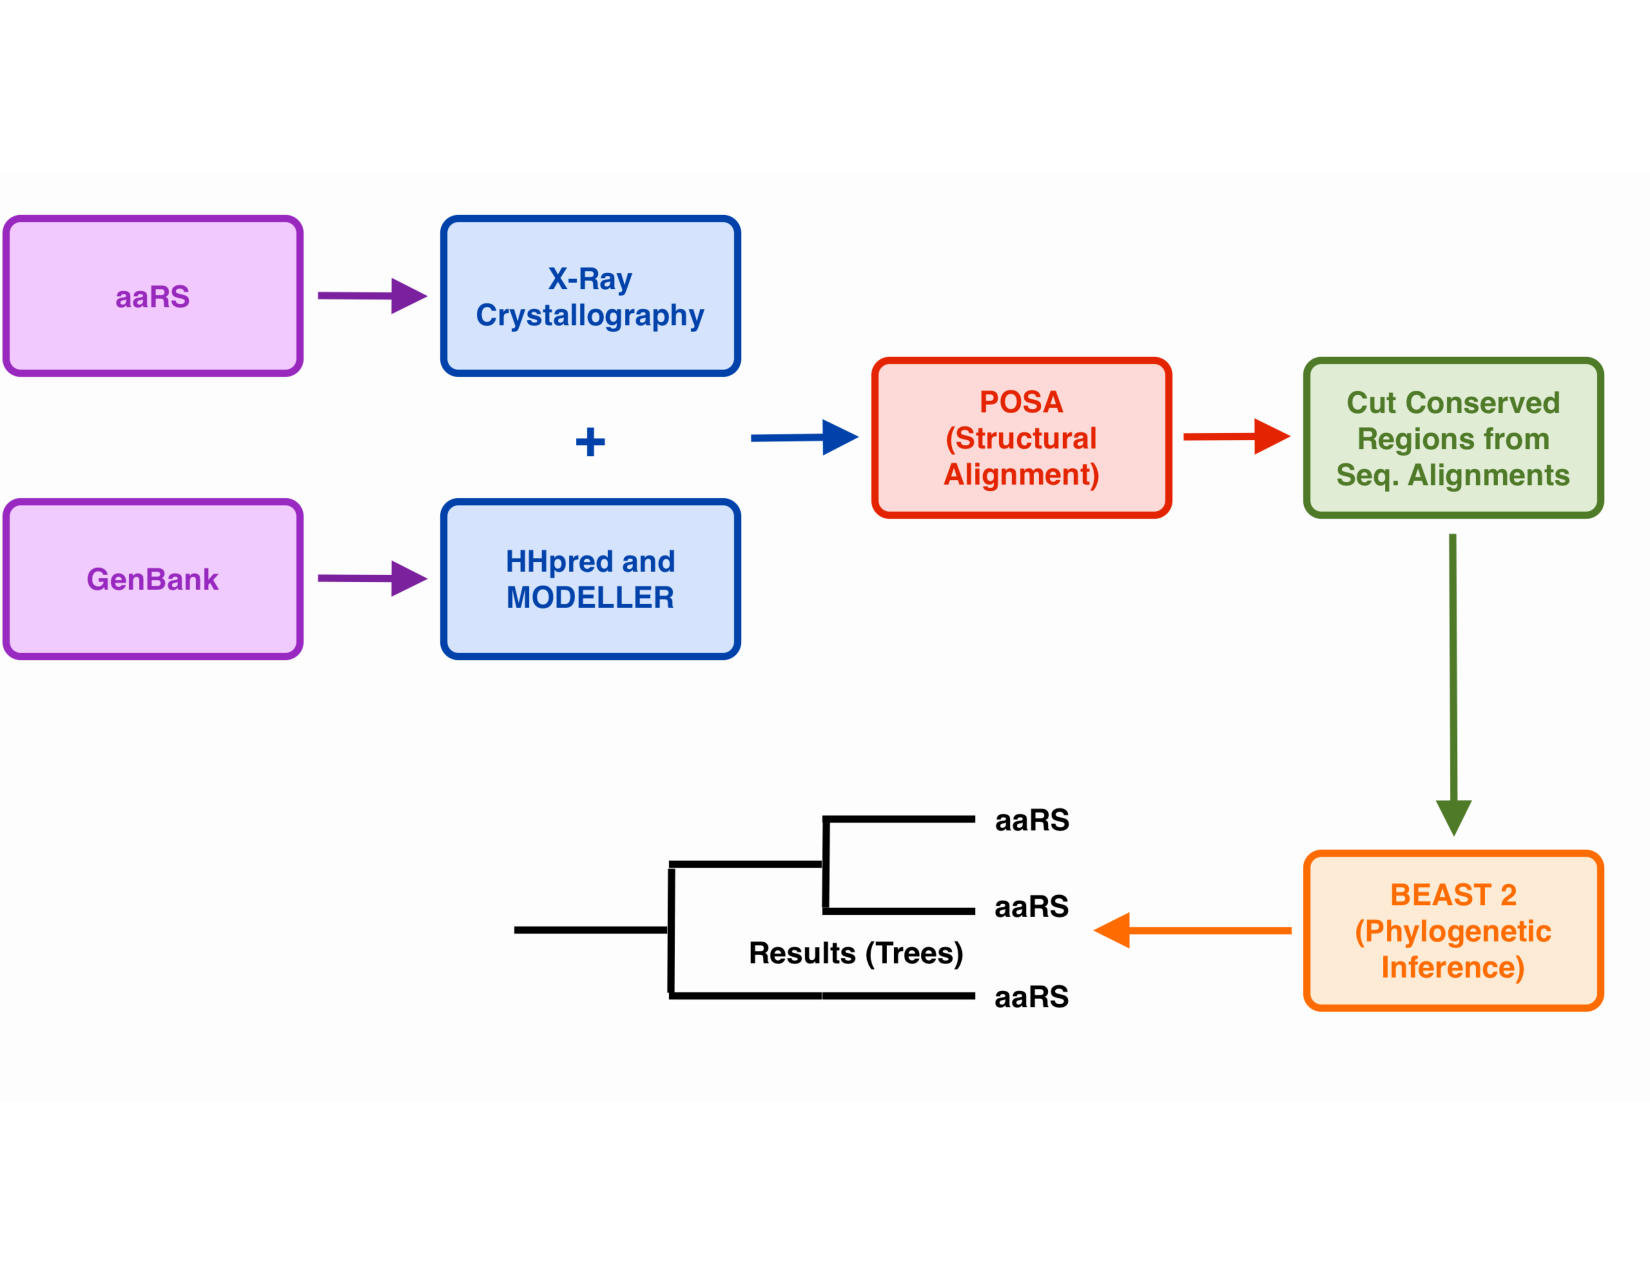
\includegraphics[width=\textwidth]{Pipeline.pdf}
  \label{pipeline}  
\end{figure}

\begin{eqnarray}
\label{eq:schemeP}
%	\mathrm{P_Y} = \underbrace{H(Y_n) - H(Y_n|\mathbf{V}^{Y}_{n})}_{S_Y} + \underbrace{H(Y_n|\mathbf{V}^{Y}_{n})- H(Y_n|\mathbf{V}^{X,Y}_{n})}_{T_{X\rightarrow Y}},
\end{eqnarray}

\section*{Materials and methods}
\subsection*{X-ray crystallography structures}



\subsection*{Modelling structures}
To ensure a statistically significant and diverse dataset, we gathered additional amino acid sequences from GenBank.  
We selected 20 organisms from each of the 3 domains of life, sampling from as many distinct clades as possible along the tips of the tree of life found in Figure \ref{treeoflife} [from: \hyperref[label_name]{``http://tolweb.org/Eukaryotes/3''}]. 
The result of our sampling is shown in Figure \ref{sampledtree}.

HHpred and Modeller


\begin{figure}
  \caption{\bf Tree of Life.  The tree from which we sampled as broadly as possible.}
  \centering
    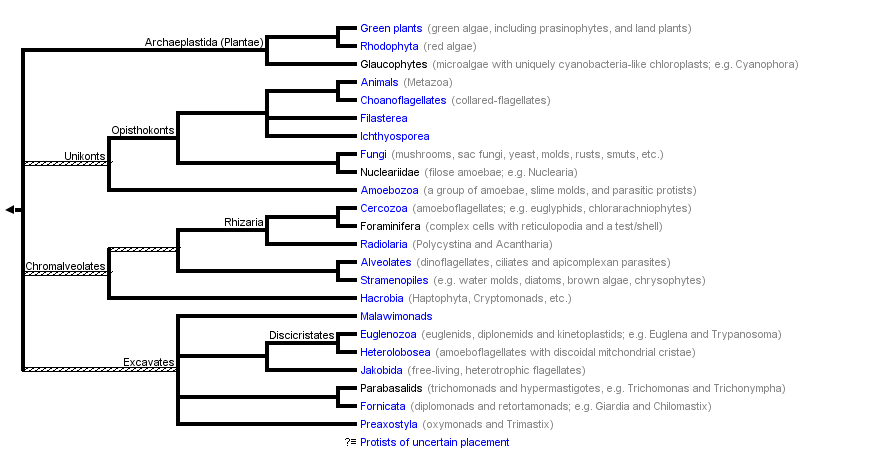
\includegraphics[width=\textwidth]{Eukaryotes.png}
  \label{treeoflife}  
\end{figure}



\subsection*{Structural alignments}


Partial Order Structure Alignment (POSA)


\subsection*{Conserved regions}


\subsection*{Phylogenetic inference}
BEAST 2




% Results and Discussion can be combined.
\section*{Results}




% Place tables after the first paragraph in which they are cited.
\begin{table}[!ht]
\scriptsize
\begin{adjustwidth}{-2.66in}{0in} % Comment out/remove adjustwidth environment if table fits in text column.
\centering
\caption{
{\bf Archaea aaRS data sampled and analysed}}
\begin{tabular}{|l+l|l|l|l|l|l|l|l|l|l|l|l|l|l|l|l|l|l|l|l|}
\hline
\multicolumn{1}{|l|}{\bf Organism} & \multicolumn{1}{|l|}{\bf ala} & \multicolumn{1}{|l|}{\bf arg} & \multicolumn{1}{|l|}{\bf asn} & \multicolumn{1}{|l|}{\bf asp} & \multicolumn{1}{|l|}{\bf cys} & \multicolumn{1}{|l|}{\bf gln} & \multicolumn{1}{|l|}{\bf glu} & \multicolumn{1}{|l|}{\bf gly} & \multicolumn{1}{|l|}{\bf his} & \multicolumn{1}{|l|}{\bf ile} & \multicolumn{1}{|l|}{\bf leu} & \multicolumn{1}{|l|}{\bf lys} & \multicolumn{1}{|l|}{\bf met} & \multicolumn{1}{|l|}{\bf phe} & \multicolumn{1}{|l|}{\bf pro} & \multicolumn{1}{|l|}{\bf ser} & \multicolumn{1}{|l|}{\bf thr} & \multicolumn{1}{|l|}{\bf trp} & \multicolumn{1}{|l|}{\bf tyr} & \multicolumn{1}{|l|}{\bf val} \\ \thickhline
$A.\ fulgidus$ & $\Theta$ & $\alpha$ & + & $\alpha$ & $\alpha$ & n/a & $\alpha$ & $\alpha$ & $\alpha$ & $\alpha$ & + & $\alpha$ & $\alpha$ & $\alpha$ & $\alpha$ & $\alpha$ & $\alpha$ & $\alpha$ & $\Theta$ & $\alpha$ \\ \hline
$A.\ pernix$ & $\alpha$ & $\alpha$ & -- & $\alpha$ & $\alpha$ & n/a & $\alpha$ & $\alpha$ & $\alpha$ & $\alpha$ & $\alpha$ & $\alpha$ & $\alpha$ & $\alpha$ & $\alpha$ & $\alpha$ & $\Theta$ & -- & $\Theta$ & $\alpha$ \\ \hline
$Halobacterium\ sp.$ & + & $\alpha$ & + & $\alpha$ & $\alpha$ & n/a & $\alpha$ & $\alpha$ & $\alpha$ & $\alpha$ & + & $\alpha$ & $\alpha$ & $\alpha$ & + & $\alpha$ & $\alpha$ & $\alpha$ & $\alpha$ & $\alpha$ \\ \hline
$M.\ acetivorans$ & $\alpha$ & $\alpha$ & + & $\alpha$ & + & n/a & + & $\alpha$ & $\alpha$ & $\alpha$ & + & $\alpha$ & $\alpha$ & $\alpha$ & $\alpha$ & $\alpha$ & $\alpha$ & $\alpha$ & $\alpha$ & $\alpha$ \\ \hline
$M.\ aeolicus\ Nankai$ & $\alpha$ & $\alpha$ & + & $\alpha$ & + & n/a & + & $\alpha$ & $\alpha$ & + & + & $\alpha$ & $\alpha$ & $\alpha$ & $\alpha$ & $\alpha$ & $\alpha$ & + & $\alpha$ & $\alpha$ \\ \hline
$M.\ barkeri$ & -- & -- & -- & -- & -- & n/a & -- & -- & -- & -- & -- & -- & -- & -- & -- & $\Theta$ & -- & -- & -- & -- \\ \hline
$M.\ hungatei$ & $\alpha$ & $\alpha$ & + & + & $\alpha$ & n/a & $\alpha$ & $\alpha$ & $\alpha$ & $\alpha$ & + & + & $\alpha$ & $\alpha$ & $\alpha$ & $\alpha$ & $\alpha$ & $\alpha$ & $\alpha$ & $\alpha$ \\ \hline
$M.\ jannaschii$ & $\alpha$ & $\alpha$ & + & $\alpha$ & -- & n/a & $\alpha$ & $\alpha$ & $\alpha$ & $\alpha$ & + & -- & $\alpha$ & $\alpha$ & $\Theta$ & $\alpha$ & $\alpha$ & $\alpha$ & $\Theta$ & $\alpha$ \\ \hline
$M.\ kandleri$ & $\alpha$ & $\alpha$ & + & $\alpha$ & + & n/a & $\alpha$ & $\alpha$ & $\alpha$ & $\alpha$ & + & $\alpha$ & $\alpha$ & $\alpha$ & $\alpha$ & $\alpha$ & $\alpha$ & $\alpha$ & $\alpha$ & $\alpha$ \\ \hline
$M.\ thermautotrophicus$ & $\alpha$ & $\alpha$ & + & $\alpha$ & + & n/a & $\alpha$ & $\alpha$ & $\alpha$ & $\alpha$ & $\alpha$ & $\alpha$ & $\alpha$ & $\alpha$ & + & $\alpha$ & $\alpha$ & $\alpha$ & $\alpha$ & $\alpha$ \\ \hline
$N.\ equitans$ & + & $\alpha$ & $\alpha$ & $\alpha$ & $\alpha$ & n/a & + & $\alpha$ & $\alpha$ & $\alpha$ & $\alpha$ & $\alpha$ & $\alpha$ & $\alpha$ & $\alpha$ & $\alpha$ & $\alpha$ & $\alpha$ & $\alpha$ & $\alpha$ \\ \hline
$P.\ abyssi$ & -- & -- & -- & -- & -- & n/a & -- & -- & -- & -- & -- & -- & $\Theta$ & -- & -- & -- & -- & -- & -- & -- \\ \hline
$P.\ aerophilum$ & + & $\alpha$ & $\alpha$ & $\alpha$ & $\alpha$ & n/a & $\alpha$ & $\alpha$ & $\alpha$ & $\alpha$ & $\alpha$ & + & $\alpha$ & $\alpha$ & $\alpha$ & $\alpha$ & $\alpha$ & $\alpha$ & $\alpha$ & $\alpha$ \\ \hline
$P.\ delaneyi$ & $\alpha$ & $\alpha$ & -- & $\alpha$ & $\alpha$ & n/a & $\alpha$ & $\alpha$ & $\alpha$ & $\alpha$ & $\alpha$ & $\alpha$ & $\alpha$ & $\alpha$ & $\alpha$ & $\alpha$ & $\alpha$ & $\alpha$ & $\alpha$ & $\alpha$ \\ \hline
$P.\ horikoshii$ & $\Theta$ & $\Theta$ & $\Theta$ & $\alpha$ & $\alpha$ & n/a & + & $\alpha$ & $\alpha$ & $\alpha$ & $\Theta$ & $\Theta$ & $\alpha$ & $\alpha$ & $\alpha$ & $\alpha$ & $\alpha$ & $\alpha$ & $\Theta$ & $\alpha$ \\ \hline
$P.\ occultum$ & $\alpha$ & $\alpha$ & -- & -- & $\alpha$ & n/a & $\alpha$ & $\alpha$ & $\alpha$ & $\alpha$ & $\alpha$ & $\alpha$ & $\alpha$ & $\alpha$ & $\alpha$ & $\alpha$ & $\alpha$ & $\alpha$ & $\alpha$ & $\alpha$ \\ \hline
$S.\ acidocaldarius$ & $\alpha$ & $\alpha$ & + & $\alpha$ & $\alpha$ & n/a & $\alpha$ & $\alpha$ & $\alpha$ & $\alpha$ & $\alpha$ & + & $\alpha$ & + & $\alpha$ & $\alpha$ & $\alpha$ & $\alpha$ & $\alpha$ & $\alpha$ \\ \hline
$S.\ marinus$ & $\alpha$ & $\alpha$ & $\alpha$ & $\alpha$ & $\alpha$ & n/a & $\alpha$ & $\alpha$ & -- & $\alpha$ & $\alpha$ & $\alpha$ & $\alpha$ & $\alpha$ & $\alpha$ & $\alpha$ & $\alpha$ & + & $\alpha$ & + \\ \hline
$S.\ tokodaii$ & -- & -- & -- & $\Theta$ & -- & n/a & -- & -- & -- & -- & -- & -- & -- & -- & -- & -- & -- & -- & -- & -- \\ \hline
$T.\ acidophilum$ & + & $\alpha$ & $\alpha$ & $\alpha$ & $\alpha$ & n/a & $\alpha$ & $\alpha$ & $\Theta$ & $\alpha$ & $\alpha$ & $\alpha$ & $\alpha$ & + & $\alpha$ & $\alpha$ & $\alpha$ & $\alpha$ & $\alpha$ & $\alpha$ \\ \hline
$T.\ kodakarensis$ & $\alpha$ & $\alpha$ & $\alpha$ & $\Theta$ & $\alpha$ & n/a & $\alpha$ & $\alpha$ & $\alpha$ & $\alpha$ & $\alpha$ & $\alpha$ & $\alpha$ & $\alpha$ & $\alpha$ & $\alpha$ & $\alpha$ & $\alpha$ & $\alpha$ & + \\ \hline
$T.\ volcanium$ & $\alpha$ & + & $\alpha$ & $\alpha$ & + & n/a & $\alpha$ & $\alpha$ & $\alpha$ & $\alpha$ & $\alpha$ & $\alpha$ & $\alpha$ & $\alpha$ & $\alpha$ & $\alpha$ & $\alpha$ & $\alpha$ & $\alpha$ & $\alpha$ \\ \hline
\end{tabular}
\begin{flushleft} \textbf{$\Theta$} means we have the crystal structures for this organism; $\alpha$ means the data was collected from Genbank, successfully modelled, and aligned; + means the data was collected from Genbank but not used in the final alignment; -- means the data was not obtained
\end{flushleft}
\label{table1}
\end{adjustwidth}
\end{table}

\begin{table}[!ht]
\scriptsize
\begin{adjustwidth}{-2.66in}{0in} % Comment out/remove adjustwidth environment if table fits in text column.
\centering
\caption{
{\bf Bacteria aaRS data sampled and analysed}}
\begin{tabular}{|l+l|l|l|l|l|l|l|l|l|l|l|l|l|l|l|l|l|l|l|l|}
\hline
\multicolumn{1}{|l|}{\bf Organism} & \multicolumn{1}{|l|}{\bf ala} & \multicolumn{1}{|l|}{\bf arg} & \multicolumn{1}{|l|}{\bf asn} & \multicolumn{1}{|l|}{\bf asp} & \multicolumn{1}{|l|}{\bf cys} & \multicolumn{1}{|l|}{\bf gln} & \multicolumn{1}{|l|}{\bf glu} & \multicolumn{1}{|l|}{\bf gly} & \multicolumn{1}{|l|}{\bf his} & \multicolumn{1}{|l|}{\bf ile} & \multicolumn{1}{|l|}{\bf leu} & \multicolumn{1}{|l|}{\bf lys} & \multicolumn{1}{|l|}{\bf met} & \multicolumn{1}{|l|}{\bf phe} & \multicolumn{1}{|l|}{\bf pro} & \multicolumn{1}{|l|}{\bf ser} & \multicolumn{1}{|l|}{\bf thr} & \multicolumn{1}{|l|}{\bf trp} & \multicolumn{1}{|l|}{\bf tyr} & \multicolumn{1}{|l|}{\bf val} \\ \thickhline
$A.\ aeolicus$ & $\Theta$ & $\alpha$ & + & $\alpha$ & $\alpha$ & + & + & + & $\alpha$ & $\alpha$ & $\alpha$ & + & $\Theta$ & $\alpha$ & $\alpha$ & $\alpha$ & $\alpha$ & $\alpha$ & $\alpha$ & + \\ \hline
$B.\ burgdorferi$ & $\alpha$ & $\alpha$ & $\alpha$ & $\alpha$ & $\alpha$ & + & $\alpha$ & $\alpha$ & $\alpha$ & $\alpha$ & $\alpha$ & + & $\alpha$ & + & $\alpha$ & $\alpha$ & $\alpha$ & $\alpha$ & $\alpha$ & $\alpha$ \\ \hline
$B.\ fragilis$ & $\alpha$ & $\alpha$ & $\alpha$ & $\alpha$ & $\alpha$ & $\alpha$ & $\alpha$ & $\alpha$ & $\alpha$ & $\alpha$ & + & $\alpha$ & $\alpha$ & + & $\alpha$ & $\alpha$ & $\alpha$ & $\alpha$ & $\alpha$ & + \\ \hline
$B.\ licheniformis$ & $\alpha$ & $\alpha$ & + & $\alpha$ & $\alpha$ & + & $\alpha$ & + & $\alpha$ & $\alpha$ & $\alpha$ & $\alpha$ & $\alpha$ & $\alpha$ & $\alpha$ & $\alpha$ & $\alpha$ & $\alpha$ & $\alpha$ & $\alpha$ \\ \hline
$B.\ thailandensis$ & $\alpha$ & $\alpha$ & + & $\alpha$ & $\alpha$ & $\alpha$ & $\alpha$ & $\alpha$ & $\alpha$ & $\alpha$ & $\alpha$ & $\alpha$ & $\alpha$ & $\alpha$ & $\alpha$ & $\alpha$ & + & $\alpha$ & + & $\alpha$ \\ \hline
$C.\ A.\ asiaticus$ & $\alpha$ & $\alpha$ & $\alpha$ & $\alpha$ & $\alpha$ & + & + & $\alpha$ & $\alpha$ & $\alpha$ & $\alpha$ & $\alpha$ & $\alpha$ & $\alpha$ & $\alpha$ & $\alpha$ & $\alpha$ & $\alpha$ & $\alpha$ & $\alpha$ \\ \hline
$C.\ aggregans$ & $\alpha$ & $\alpha$ & $\alpha$ & $\alpha$ & $\alpha$ & + & $\alpha$ & $\alpha$ & $\alpha$ & $\alpha$ & $\alpha$ & $\alpha$ & $\alpha$ & $\alpha$ & $\alpha$ & $\alpha$ & $\alpha$ & $\alpha$ & $\alpha$ & + \\ \hline
$C.\ jejuni$ & + & $\Theta$ & + & $\alpha$ & $\alpha$ & $\alpha$ & $\alpha$ & + & $\alpha$ & $\alpha$ & $\alpha$ & $\alpha$ & $\alpha$ & $\alpha$ & + & $\alpha$ & $\alpha$ & $\alpha$ & $\alpha$ & $\alpha$ \\ \hline
$C.\ thermalis$ & $\alpha$ & $\alpha$ & $\alpha$ & + & $\alpha$ & + & + & + & $\alpha$ & $\alpha$ & $\alpha$ & + & $\alpha$ & $\alpha$ & $\alpha$ & $\alpha$ & $\alpha$ & $\alpha$ & $\alpha$ & $\alpha$ \\ \hline
$D.\ radiodurans$ & $\alpha$ & $\alpha$ & $\alpha$ & $\alpha$ & $\alpha$ & $\Theta$ & $\alpha$ & $\alpha$ & $\alpha$ & $\alpha$ & $\alpha$ & $\alpha$ & $\alpha$ & $\alpha$ & $\alpha$ & $\alpha$ & $\alpha$ & $\alpha$ & $\alpha$ & $\alpha$ \\ \hline
$E.\ coli$ & $\Theta$ & $\alpha$ & $\alpha$ & $\Theta$ & $\Theta$ & $\Theta$ & $\Theta$ & $\Theta$ & $\Theta$ & $\alpha$ & $\alpha$ & $\Theta$ & $\Theta$ & $\alpha$ & $\alpha$ & $\alpha$ & $\Theta$ & $\alpha$ & $\Theta$ & $\alpha$ \\ \hline
$E.\ faecalis$ & $\alpha$ & $\alpha$ & $\alpha$ & $\alpha$ & $\alpha$ & -- & $\alpha$ & $\alpha$ & $\alpha$ & $\alpha$ & $\alpha$ & $\alpha$ & $\alpha$ & $\alpha$ & $\Theta$ & $\alpha$ & $\alpha$ & $\alpha$ & $\alpha$ & $\alpha$ \\ \hline
$G.\ obscuriglobus$ & $\alpha$ & $\alpha$ & $\alpha$ & + & $\alpha$ & $\alpha$ & $\alpha$ & $\alpha$ & $\alpha$ & $\alpha$ & $\alpha$ & $\alpha$ & $\alpha$ & $\alpha$ & $\alpha$ & + & $\alpha$ & $\alpha$ & $\alpha$ & + \\ \hline
$G.\ stearothermophilus$ & $\alpha$ & $\alpha$ & + & $\alpha$ & + & $\alpha$ & $\alpha$ & $\alpha$ & $\alpha$ & $\alpha$ & $\alpha$ & $\Theta$ & $\alpha$ & -- & $\alpha$ & $\alpha$ & $\alpha$ & $\Theta$ & $\alpha$ & $\alpha$ \\ \hline
$H.\ aurantiacus$ & $\alpha$ & $\alpha$ & $\alpha$ & $\alpha$ & $\alpha$ & -- & $\alpha$ & $\alpha$ & $\alpha$ & $\alpha$ & + & $\alpha$ & $\alpha$ & $\alpha$ & $\alpha$ & $\alpha$ & $\alpha$ & $\alpha$ & $\alpha$ & + \\ \hline
$M.\ mobile$ & $\alpha$ & + & $\alpha$ & $\alpha$ & $\alpha$ & -- & $\Theta$ & $\alpha$ & $\alpha$ & $\alpha$ & $\alpha$ & $\alpha$ & + & $\alpha$ & + & $\alpha$ & + & + & $\alpha$ & $\alpha$ \\ \hline
$M.\ smegmatis$ & + & + & + & $\alpha$ & $\Theta$ & + & + & + & + & + & $\alpha$ & + & $\alpha$ & $\alpha$ & + & $\alpha$ & + & + & + & $\alpha$ \\ \hline
$P.\ mikurensis$ & $\alpha$ & $\alpha$ & -- & $\alpha$ & $\alpha$ & $\alpha$ & $\alpha$ & $\alpha$ & $\alpha$ & $\alpha$ & + & $\alpha$ & $\alpha$ & $\alpha$ & $\alpha$ & + & $\alpha$ & $\alpha$ & $\alpha$ & + \\ \hline
$R.\ marinus$ & + & $\alpha$ & $\alpha$ & $\alpha$ & $\alpha$ & -- & $\alpha$ & $\alpha$ & $\alpha$ & $\alpha$ & + & + & $\alpha$ & $\alpha$ & $\alpha$ & $\alpha$ & $\alpha$ & $\alpha$ & * & $\alpha$ \\ \hline
$R.\ palustris$ & $\alpha$ & $\alpha$ & -- & $\alpha$ & $\alpha$ & $\alpha$ & + & $\alpha$ & $\alpha$ & + & + & $\alpha$ & $\alpha$ & $\alpha$ & $\Theta$ & $\alpha$ & $\alpha$ & $\alpha$ & $\alpha$ & $\alpha$ \\ \hline
$S.\ aureus$ & $\alpha$ & $\alpha$ & $\alpha$ & $\alpha$ & $\alpha$ & + & + & $\Theta$ & $\Theta$ & $\Theta$ & $\alpha$ & $\alpha$ & $\alpha$ & $\alpha$ & $\alpha$ & $\alpha$ & $\Theta$ & $\alpha$ & $\Theta$ & $\alpha$ \\ \hline
$S.\ elongatus$ & $\alpha$ & $\alpha$ & $\alpha$ & $\alpha$ & $\alpha$ & $\alpha$ & $\Theta$ & $\alpha$ & $\alpha$ & $\alpha$ & $\alpha$ & $\alpha$ & $\alpha$ & + & $\alpha$ & $\alpha$ & $\alpha$ & $\alpha$ & $\alpha$ & $\alpha$ \\ \hline
$S.\ haemolyticus$ & $\alpha$ & $\alpha$ & $\alpha$ & $\alpha$ & $\alpha$ & -- & $\alpha$ & $\alpha$ & $\alpha$ & $\alpha$ & $\alpha$ & $\alpha$ & $\alpha$ & $\Theta$ & $\alpha$ & $\alpha$ & $\alpha$ & $\alpha$ & $\alpha$ & $\alpha$ \\ \hline
$S.\ typhimurium$ & -- & -- & -- & -- & -- & -- & -- & -- & -- & -- & -- & $\Theta$ & -- & -- & -- & -- & -- & -- & -- & -- \\ \hline
$T.\ maritima$ & $\alpha$ & $\alpha$ & + & $\alpha$ & $\alpha$ & $\Theta$ & $\Theta$ & $\Theta$ & $\alpha$ & $\alpha$ & $\alpha$ & $\alpha$ & $\alpha$ & -- & $\alpha$ & $\alpha$ & $\alpha$ & $\Theta$ & $\alpha$ & $\alpha$ \\ \hline
$T.\ thermophilus$ & $\alpha$ & $\Theta$ & $\Theta$ & $\Theta$ & $\alpha$ & $\Theta$ & $\Theta$ & $\Theta$ & $\Theta$ & $\Theta$ & $\Theta$ & $\alpha$ & $\Theta$ & $\Theta$ & $\Theta$ & $\Theta$ & $\alpha$ & $\Theta$ & $\Theta$ & $\Theta$ \\ \hline
\end{tabular}
\begin{flushleft} \textbf{$\Theta$} means we have the crystal structures for this organism; $\alpha$ means the data was collected from Genbank, successfully modelled, and aligned; + means the data was collected from Genbank but not used in the final alignment; -- means the data was not obtained
\end{flushleft}
\label{table1}
\end{adjustwidth}
\end{table}

\begin{table}[!ht]
\scriptsize
\begin{adjustwidth}{-2.56in}{0in} % Comment out/remove adjustwidth environment if table fits in text column.
\centering
\caption{
{\bf Eukaryote aaRS data sampled and analysed}}
\begin{tabular}{|l+l|l|l|l|l|l|l|l|l|l|l|l|l|l|l|l|l|l|l|l|}
\hline
\multicolumn{1}{|l|}{\bf Organism} & \multicolumn{1}{|l|}{\bf ala} & \multicolumn{1}{|l|}{\bf arg} & \multicolumn{1}{|l|}{\bf asn} & \multicolumn{1}{|l|}{\bf asp} & \multicolumn{1}{|l|}{\bf cys} & \multicolumn{1}{|l|}{\bf gln} & \multicolumn{1}{|l|}{\bf glu} & \multicolumn{1}{|l|}{\bf gly} & \multicolumn{1}{|l|}{\bf his} & \multicolumn{1}{|l|}{\bf ile} & \multicolumn{1}{|l|}{\bf leu} & \multicolumn{1}{|l|}{\bf lys} & \multicolumn{1}{|l|}{\bf met} & \multicolumn{1}{|l|}{\bf phe} & \multicolumn{1}{|l|}{\bf pro} & \multicolumn{1}{|l|}{\bf ser} & \multicolumn{1}{|l|}{\bf thr} & \multicolumn{1}{|l|}{\bf trp} & \multicolumn{1}{|l|}{\bf tyr} & \multicolumn{1}{|l|}{\bf val} \\ \thickhline
$A.\ subglabra$ & -- & $\alpha$ & $\alpha$ & $\alpha$ & -- & $\alpha$ & $\alpha$ & $\alpha$ & $\alpha$ & $\alpha$ & $\alpha$ & $\alpha$ & $\alpha$ & + & $\alpha$ & $\alpha$ & $\alpha$ & $\alpha$ & $\alpha$ & -- \\ \hline
$B.\ hominis$ & $\alpha$ & -- & -- & $\alpha$ & $\alpha$ & -- & $\alpha$ & $\alpha$ & -- & $\alpha$ & $\alpha$ & $\alpha$ & $\alpha$ & $\alpha$ & $\alpha$ & -- & -- & -- & $\alpha$ & $\alpha$ \\ \hline
$B.\ mori$ & $\alpha$ & $\Theta$ & $\alpha$ & $\alpha$ & -- & -- & $\alpha$ & $\alpha$ & -- & $\alpha$ & -- & $\alpha$ & $\alpha$ & $\alpha$ & + & $\alpha$ & $\alpha$ & $\alpha$ & -- & -- \\ \hline
$B.\ taurus$ & + & + & + & -- & + & -- & + & + & + & + & $\alpha$ & + & + & + & + & $\Theta$ & + & $\alpha$ & + & + \\ \hline
$C.\ gigas$ & $\alpha$ & + & $\alpha$ & $\alpha$ & $\alpha$ & $\alpha$ & + & $\alpha$ & $\alpha$ & $\alpha$ & $\alpha$ & $\alpha$ & $\alpha$ & $\alpha$ & $\alpha$ & $\alpha$ & $\alpha$ & $\alpha$ & $\alpha$ & $\alpha$ \\ \hline
$C.\ owczarzaki$ & $\alpha$ & $\alpha$ & $\alpha$ & $\alpha$ & $\alpha$ & $\alpha$ & + & $\alpha$ & $\alpha$ & $\alpha$ & $\alpha$ & $\alpha$ & + & + & $\alpha$ & $\alpha$ & $\alpha$ & $\alpha$ & $\alpha$ & $\alpha$ \\ \hline
$C.\ parvum\ Iowa\ II$ & $\alpha$ & -- & $\alpha$ & $\alpha$ & $\alpha$ & $\alpha$ & $\alpha$ & $\alpha$ & $\alpha$ & $\alpha$ & -- & $\alpha$ & $\alpha$ & + & $\alpha$ & $\alpha$ & + & $\alpha$ & $\alpha$ & $\alpha$ \\ \hline
$C.\ subellipsoidea$ & $\alpha$ & $\alpha$ & + & $\alpha$ & -- & $\alpha$ & -- & $\alpha$ & + & $\alpha$ & $\alpha$ & $\alpha$ & $\alpha$ & + & $\alpha$ & $\alpha$ & $\alpha$ & + & $\alpha$ & $\alpha$ \\ \hline
$D.\ discoideum$ & $\alpha$ & $\alpha$ & $\alpha$ & $\alpha$ & $\alpha$ & -- & + & $\alpha$ & $\alpha$ & $\alpha$ & + & $\alpha$ & $\alpha$ & $\alpha$ & $\alpha$ & $\alpha$ & $\alpha$ & $\alpha$ & $\alpha$ & $\alpha$ \\ \hline
$D.\ rerio$ & $\alpha$ & $\alpha$ & + & -- & + & $\alpha$ & $\alpha$ & + & $\alpha$ & + & + & -- & + & + & + & + & + & $\alpha$ & + & $\alpha$ \\ \hline
$E.\ guttata$ & $\alpha$ & + & + & $\alpha$ & $\alpha$ & $\alpha$ & $\alpha$ & -- & $\alpha$ & $\alpha$ & $\alpha$ & + & $\alpha$ & $\alpha$ & $\alpha$ & $\alpha$ & $\alpha$ & $\alpha$ & + & $\alpha$ \\ \hline
$E.\ histolytica$ & $\alpha$ & + & $\Theta$ & $\Theta$ & $\alpha$ & $\alpha$ & $\alpha$ & $\alpha$ & $\alpha$ & $\alpha$ & + & -- & $\alpha$ & $\alpha$ & $\alpha$ & $\alpha$ & $\alpha$ & $\alpha$ & $\alpha$ & $\alpha$ \\ \hline
$G.\ lamblia$ & + & $\alpha$ & $\alpha$ & $\alpha$ & $\alpha$ & $\alpha$ & -- & $\alpha$ & $\alpha$ & $\alpha$ & $\alpha$ & $\alpha$ & $\alpha$ & $\alpha$ & $\Theta$ & $\alpha$ & $\alpha$ & $\alpha$ & $\alpha$ & $\alpha$ \\ \hline
$G.\ theta$ & $\alpha$ & $\alpha$ & $\alpha$ & $\alpha$ & $\alpha$ & $\alpha$ & + & $\alpha$ & $\alpha$ & $\alpha$ & $\alpha$ & $\alpha$ & $\alpha$ & $\alpha$ & $\alpha$ & $\alpha$ & $\alpha$ & $\alpha$ & $\alpha$ & + \\ \hline
$H.\ sapiens$ & + & + & $\alpha$ & -- & -- & $\Theta$ & $\alpha$ & $\Theta$ & $\alpha$ & $\alpha$ & $\alpha$ & $\Theta$ & $\alpha$ & $\Theta$ & + & $\alpha$ & $\alpha$ & $\Theta$ & $\alpha$ & -- \\ \hline
$L.\ infantum$ & $\alpha$ & $\alpha$ & $\alpha$ & $\alpha$ & $\alpha$ & $\alpha$ & $\alpha$ & $\alpha$ & $\alpha$ & $\alpha$ & $\alpha$ & $\alpha$ & $\alpha$ & $\alpha$ & $\alpha$ & $\alpha$ & $\alpha$ & $\alpha$ & $\alpha$ & $\alpha$ \\ \hline
$M.\ domestica$ & + & $\alpha$ & + & + & + & $\alpha$ & + & + & $\alpha$ & + & + & + & + & $\alpha$ & + & + & + & $\alpha$ & $\alpha$ & $\alpha$ \\ \hline
$N.\ ceranae$ & $\alpha$ & $\alpha$ & $\alpha$ & $\alpha$ & $\alpha$ & $\alpha$ & $\alpha$ & $\alpha$ & + & $\alpha$ & $\alpha$ & $\alpha$ & $\alpha$ & + & $\alpha$ & $\alpha$ & $\alpha$ & $\alpha$ & $\alpha$ & $\alpha$ \\ \hline
$N.\ gruberi$ & $\alpha$ & -- & $\alpha$ & $\alpha$ & $\alpha$ & -- & -- & $\alpha$ & -- & $\alpha$ & + & $\alpha$ & $\alpha$ & $\alpha$ & $\alpha$ & $\alpha$ & $\alpha$ & $\alpha$ & $\alpha$ & $\alpha$ \\ \hline
$P.\ bivittatus$ & + & + & + & + & $\alpha$ & + & + & + & + & + & + & + & + & + & + & + & -- & + & + & + \\ \hline
$P.\ chromatophora$ & $\alpha$ & $\alpha$ & -- & $\alpha$ & $\alpha$ & -- & $\alpha$ & + & $\alpha$ & $\alpha$ & $\alpha$ & $\alpha$ & $\alpha$ & $\alpha$ & $\alpha$ & $\alpha$ & $\alpha$ & $\alpha$ & $\alpha$ & $\alpha$ \\ \hline
$P.\ euphratica$ & + & $\alpha$ & $\alpha$ & -- & + & + & -- & -- & + & + & + & + & + & + & + & + & + & + & + & + \\ \hline
$S.\ cerevisiae$ & -- & $\Theta$ & -- & -- & -- & -- & -- & -- & -- & -- & -- & -- & -- & -- & -- & -- & -- & $\Theta$ & $\Theta$ & -- \\ \hline
$S.\ rosetta$ & $\alpha$ & $\alpha$ & $\alpha$ & $\alpha$ & $\alpha$ & $\alpha$ & $\alpha$ & $\alpha$ & -- & $\alpha$ & + & $\alpha$ & $\alpha$ & $\alpha$ & $\alpha$ & $\alpha$ & $\alpha$ & + & $\alpha$ & $\alpha$ \\ \hline
$R.\ filosa$ & + & -- & + & -- & + & + & + & + & -- & -- & + & + & + & $\alpha$ & $\alpha$ & + & $\alpha$ & + & -- & -- \\ \hline
$T.\ brucei$ & -- & -- & -- & -- & -- & -- & -- & -- & $\Theta$ & -- & -- & + & + & -- & -- & -- & -- & + & + & -- \\ \hline
$T.\ cruzi$ & -- & -- & -- & -- & -- & -- & -- & -- & $\Theta$ & -- & -- & -- & -- & -- & -- & -- & -- & -- & -- & -- \\ \hline
$T.\ vaginalis$ & + & -- & $\alpha$ & -- & $\alpha$ & $\alpha$ & $\alpha$ & $\alpha$ & $\alpha$ & $\alpha$ & $\alpha$ & $\alpha$ & -- & $\alpha$ & $\alpha$ & $\alpha$ & $\alpha$ & $\alpha$ & -- & + \\ \hline
\end{tabular}
\begin{flushleft} \textbf{$\Theta$} means we have the crystal structures for this organism; $\alpha$ means the data was collected from Genbank, successfully modelled, and aligned; + means the data was collected from Genbank but not used in the final alignment; -- means the data was not obtained
\end{flushleft}
\label{table1}
\end{adjustwidth}
\end{table}

% T. BRUCEI TYR/MET???

TREE ANNOTATOR + FIGTREE

TREESTAT

RELAXED CLOCK

%PLOS does not support heading levels beyond the 3rd (no 4th level headings).
\subsection*{\lorem\ and \ipsum\ nunc blandit a tortor}
\subsubsection*{3rd level heading} 
Maecenas convallis mauris sit amet sem ultrices gravida.

\begin{enumerate}
	\item{react}
	\item{diffuse free particles}
	\item{increment time by dt and go to 1}
\end{enumerate}


\subsection*{Sed ac quam id nisi malesuada congue}

Nulla mi mi, venenatis sed ipsum varius, volutpat euismod diam. 



\section*{Discussion}
Nulla mi mi, venenatis sed ipsum varius, Table~\ref{table1} 

\section*{Conclusion}

%CO\textsubscript{2} Maecenas convallis mauris sit amet sem ultrices gravida. Etiam eget sapien nibh. Sed ac ipsum eget enim egestas ullamcorper nec euismod ligula. Curabitur fringilla pulvinar lectus consectetur pellentesque. Quisque augue sem, tincidunt sit amet feugiat eget, ullamcorper sed velit. 

Sed non aliquet felis. , see \nameref{S1_Appendix}.

\section*{Supporting information}

Here we provide details of the organisms we sampled for the aaRS Class I and Class II phylogenies.

\begin{figure}
  \caption{\bf Tree of Life.  Tree showing our sampling efficacy.}
  \centering
    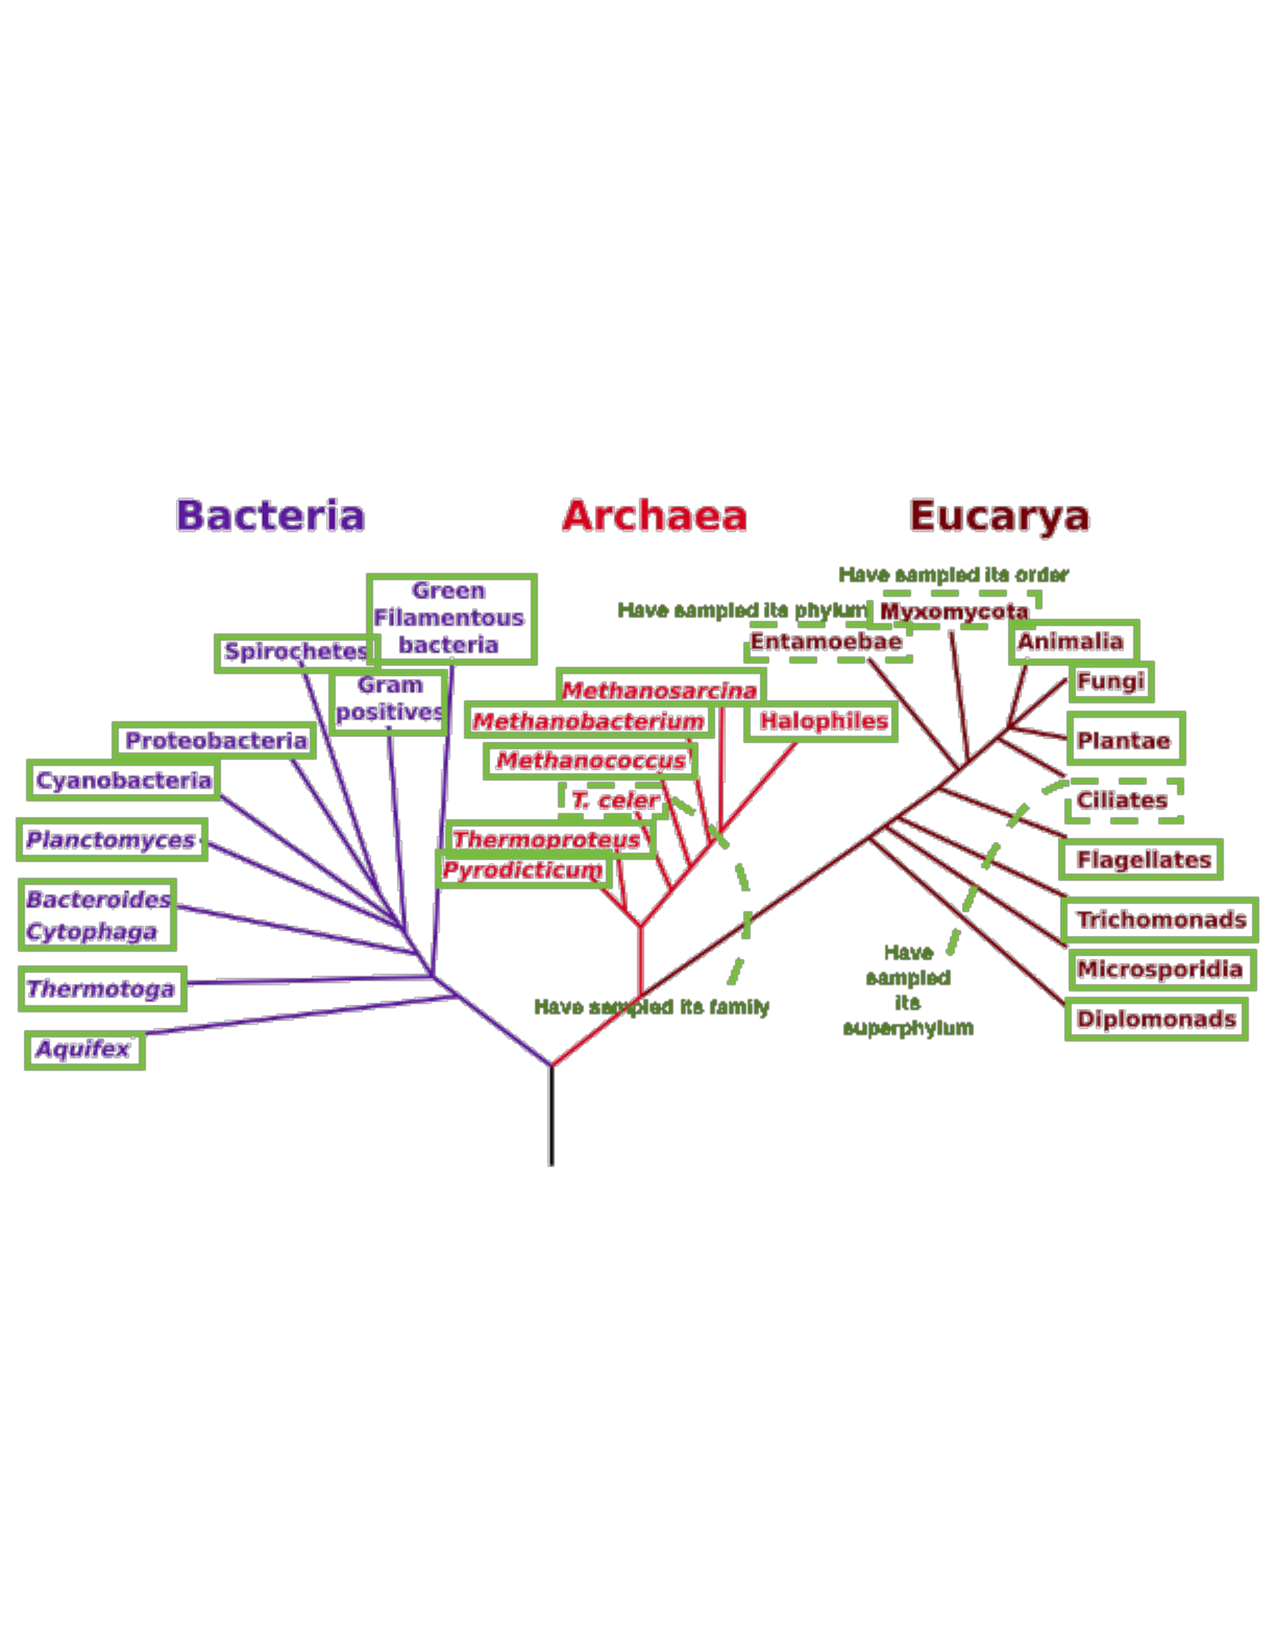
\includegraphics[width=\textwidth]{TreeofLife.pdf}
  \label{sampledtree}  
\end{figure}

Archaea

\begin{itemize}
	\item Methanosarcina
	\begin{itemize}
		\item \textit{Methanosarcina acetivorans}
		\item \textit{Methanosarcina barkeri}
	\end{itemize}
	\item Halophiles
	\begin{itemize}
		\item \textit{Halobacterium sp.}
	\end{itemize}
	\item Methanobacterium
	\begin{itemize}
		\item \textit{Methanothermobacter thermautotrophicus}
	\end{itemize}
	\item Methanococcus
	\begin{itemize}
		\item \textit{Methanococcus aeolicus Nankai}
		\item \textit{Methanococcus jannaschii}
	\end{itemize}
	\item Thermococcus
	\begin{itemize}
		\item \textit{Pyrococcus horikoshii}
		\item \textit{Pyrococcus abyssi}
		\item \textit{Thermococcus kodakarensis}
	\end{itemize}
	\item Thermoproteus
	\begin{itemize}
		\item \textit{Pyrobaculum aerophilum}
		\item \textit{Staphylothermus marinus}
		\item \textit{Sulfolobus acidocaldarius}
		\item \textit{Aeropyrum pernix}
		\item \textit{Sulfolobus tokodaii}
	\end{itemize}
	\item Pyrodicticum
	\begin{itemize}
		\item \textit{Pyrodictium occultum}
		\item \textit{Pyrodictium delaneyi}
	\end{itemize}
	\item Other
	\begin{itemize}
		\item \textit{Methanospirillum hungatei}
		\item \textit{Nanoarchaeum equitans}
		\item \textit{Thermoplasma volcanium}
		\item \textit{Thermoplasma acidophilum}
		\item \textit{Methanopyrus kandleri}
		\item \textit{Archaeoglobus fulgidus}
	\end{itemize}
\end{itemize}

Bacteria

\begin{itemize}
	\item ``Green filamentous bacteria''
	\begin{itemize}
		\item \textit{Chloroflexus aggregans}
		\item \textit{Herpetosiphon aurantiacus}
	\end{itemize}
	\item Gram positives
	\begin{itemize}
		\item \textit{Bacillus licheniformis}
		\item \textit{Geobacillus stearothermophilus}
		\item \textit{Mycobacterium smegmatis}
		\item \textit{Mycoplasma mobile}
		\item \textit{Staphylococcus aureus}
	\end{itemize}
	\item Spirochetes
	\begin{itemize}
		\item \textit{Borrelia burgdorferi}
	\end{itemize}
	\item Proteobacteria
	\begin{itemize}
		\item \textit{Burkholderia thailandensis}
		\item \textit{Campylobacter jejuni}
		\item \textit{Escherichia coli}
		\item \textit{Rhodopseudomonas palustris}
		\item \textit{Salmonella typhimurium}
	\end{itemize}
	\item Cyanobacteria
	\begin{itemize}
		\item \textit{Synechococcus elongatus}
		\item \textit{Chroococcidiopsis thermalis}
	\end{itemize}
	\item Plantomycetes
	\begin{itemize}
		\item \textit{Phycisphaera mikurensis}
		\item \textit{Gemmata obscuriglobus}
	\end{itemize}
	\item Bacteroides/Cytophaga
	\begin{itemize}
		\item \textit{Candidatus Amoebophilus asiaticus}
		\item \textit{Bacteroides fragilis}
	\end{itemize}
	\item Thermotoga
	\begin{itemize}
		\item \textit{Thermotoga maritima}
	\end{itemize}
	\item Aquifex
	\begin{itemize}
		\item \textit{Aquifex aeolicus}
	\end{itemize}
	\item Other
	\begin{itemize}
		\item \textit{Deinococcus radiodurans}
		\item \textit{Thermus thermophilus}
		\item \textit{Enterococcus faecalis}
		\item \textit{Rhodothermus marinus}
		\item \textit{Staphylococcus haemolyticus}
	\end{itemize}
\end{itemize}


Eukarya

\begin{itemize}
	\item Entamoebae/Myxomycota
	\begin{itemize}
		\item \textit{Dictyostelium discoideum} (soil-living amoeba, slime mold)
		\item \textit{Entamoeba histolytica} (anaerobic parasitic amoebozoa)
	\end{itemize}
	\item Animalia
	\begin{itemize}
		\item \textit{Homo sapiens} (human)
		\item \textit{Bos taurus} (cattle)
		\item \textit{Danio rerio} (zebrafish)
		\item \textit{Python bivittatus} (Burmese python)
		\item \textit{Bombyx mori} (silkworm)
		\item \textit{Musca domestica} (housefly)
		\item \textit{Crassostrea gigas} (Pacific oyster)
	\end{itemize}
	\item Fungi
	\begin{itemize}
		\item \textit{Auricularia subglabra} (jelly fungi)
		\item \textit{Saccharomyces cerevisiae} (yeast)
	\end{itemize}
	\item Plantae
	\begin{itemize}
		\item \textit{Erythranthe guttata} (yellow monkey flower)
		\item \textit{Populus euphratica} (Euphrates or desert poplar)
		\item Green algae
		\begin{itemize}
			\item \textit{Coccomyxa subellipsoidea} (green algae)
		\end{itemize}
	\end{itemize}
	\item Ciliates
	\begin{itemize}
		\item \textit{Cryptosporidium parvum Iowa II} (apicomplexan protozoan)
	\end{itemize}
	\item Flagellates
	\begin{itemize}
			\item \textit{Guillardia theta} (flagellate cryptomonad algae)
			\item \textit{Salpingoeca rosetta} (choanoflagellate, closest living relatives of the animals)
			\item \textit{Leishmania infantum} (kinetoplastid protozoan with single flagellum)
			\item Diplomonads
			\begin{itemize}
				\item \textit{Giardia lamblia} (flagellated protozoan parasite)
			\end{itemize}
			\item Trichomonads
			\begin{itemize}
				\item \textit{Trichomonas vaginalis} (anaerobic, flagellated protozoan parasite)
			\end{itemize}
	\end{itemize}
	\item Microsporidia
	\begin{itemize}
		\item \textit{Nosema ceranae} (unicellular honey bee parasite)
	\end{itemize}
	\item Etc.
	\begin{itemize}
		\item \textit{Naegleria gruberi} (famous for ability to change from amoeba to flagellate)
		\item \textit{Blastocystis hominis} (single-celled protozoan human parasite)
		\item \textit{Reticulomyxa filosa} (freshwater foraminifer with anastamozing pseudopodia)
		\item \textit{Capsaspora owczarzaki} (single-celled amoeba symbiont with tropical freshwater snail)
		\item \textit{Paulinella chromatophora} (photosynthetic freshwater amoeba)
		\item \textit{Trypanosoma brucei} (parasite, causes sleeping sickness)
		\item \textit{Trypanosoma cruzi} (parasite, causes Chagas disease)
	\end{itemize}
\end{itemize}

% Include only the SI item label in the paragraph heading. Use the \nameref{label} command to cite SI items in the text.
\paragraph*{S1 Fig.}
\label{S1_Fig}
{\bf Bold the title sentence.} Add descriptive text after the title of the item (optional).

\paragraph*{S2 Fig.}
\label{S2_Fig}
{\bf Lorem ipsum.} Maecenas convallis mauris sit amet sem ultrices gravida. Etiam eget sapien nibh. Sed ac ipsum eget enim egestas ullamcorper nec euismod ligula. Curabitur fringilla pulvinar lectus consectetur pellentesque.

\paragraph*{S1 File.}
\label{S1_File}
{\bf Lorem ipsum.}  Maecenas convallis mauris sit amet sem ultrices gravida. Etiam eget sapien nibh. Sed ac ipsum eget enim egestas ullamcorper nec euismod ligula. Curabitur fringilla pulvinar lectus consectetur pellentesque.

\paragraph*{S1 Video.}
\label{S1_Video}
{\bf Lorem ipsum.}  Maecenas convallis mauris sit amet sem ultrices gravida. Etiam eget sapien nibh. Sed ac ipsum eget enim egestas ullamcorper nec euismod ligula. Curabitur fringilla pulvinar lectus consectetur pellentesque.

\paragraph*{S1 Appendix.}
\label{S1_Appendix}
{\bf Lorem ipsum.} Maecenas convallis mauris sit amet sem ultrices gravida. Etiam eget sapien nibh. Sed ac ipsum eget enim egestas ullamcorper nec euismod ligula. Curabitur fringilla pulvinar lectus consectetur pellentesque.

\paragraph*{S1 Table.}
\label{S1_Table}
{\bf Lorem ipsum.} Maecenas convallis mauris sit amet sem ultrices gravida. Etiam eget sapien nibh. Sed ac ipsum eget enim egestas ullamcorper nec euismod ligula. Curabitur fringilla pulvinar lectus consectetur pellentesque.

\section*{Acknowledgments}
Cras egestas velit mauris, eu mollis turpis pellentesque sit amet. Interdum et malesuada fames ac ante ipsum primis in faucibus. Nam id pretium nisi. Sed ac quam id nisi malesuada congue. Sed interdum aliquet augue, at pellentesque quam rhoncus vitae.

\nolinenumbers

%
% FIGURES
%
\begin{figure}
  \caption{\bf Class I consensus tree with coalescent tree prior and strict clock model.}
  \centering
    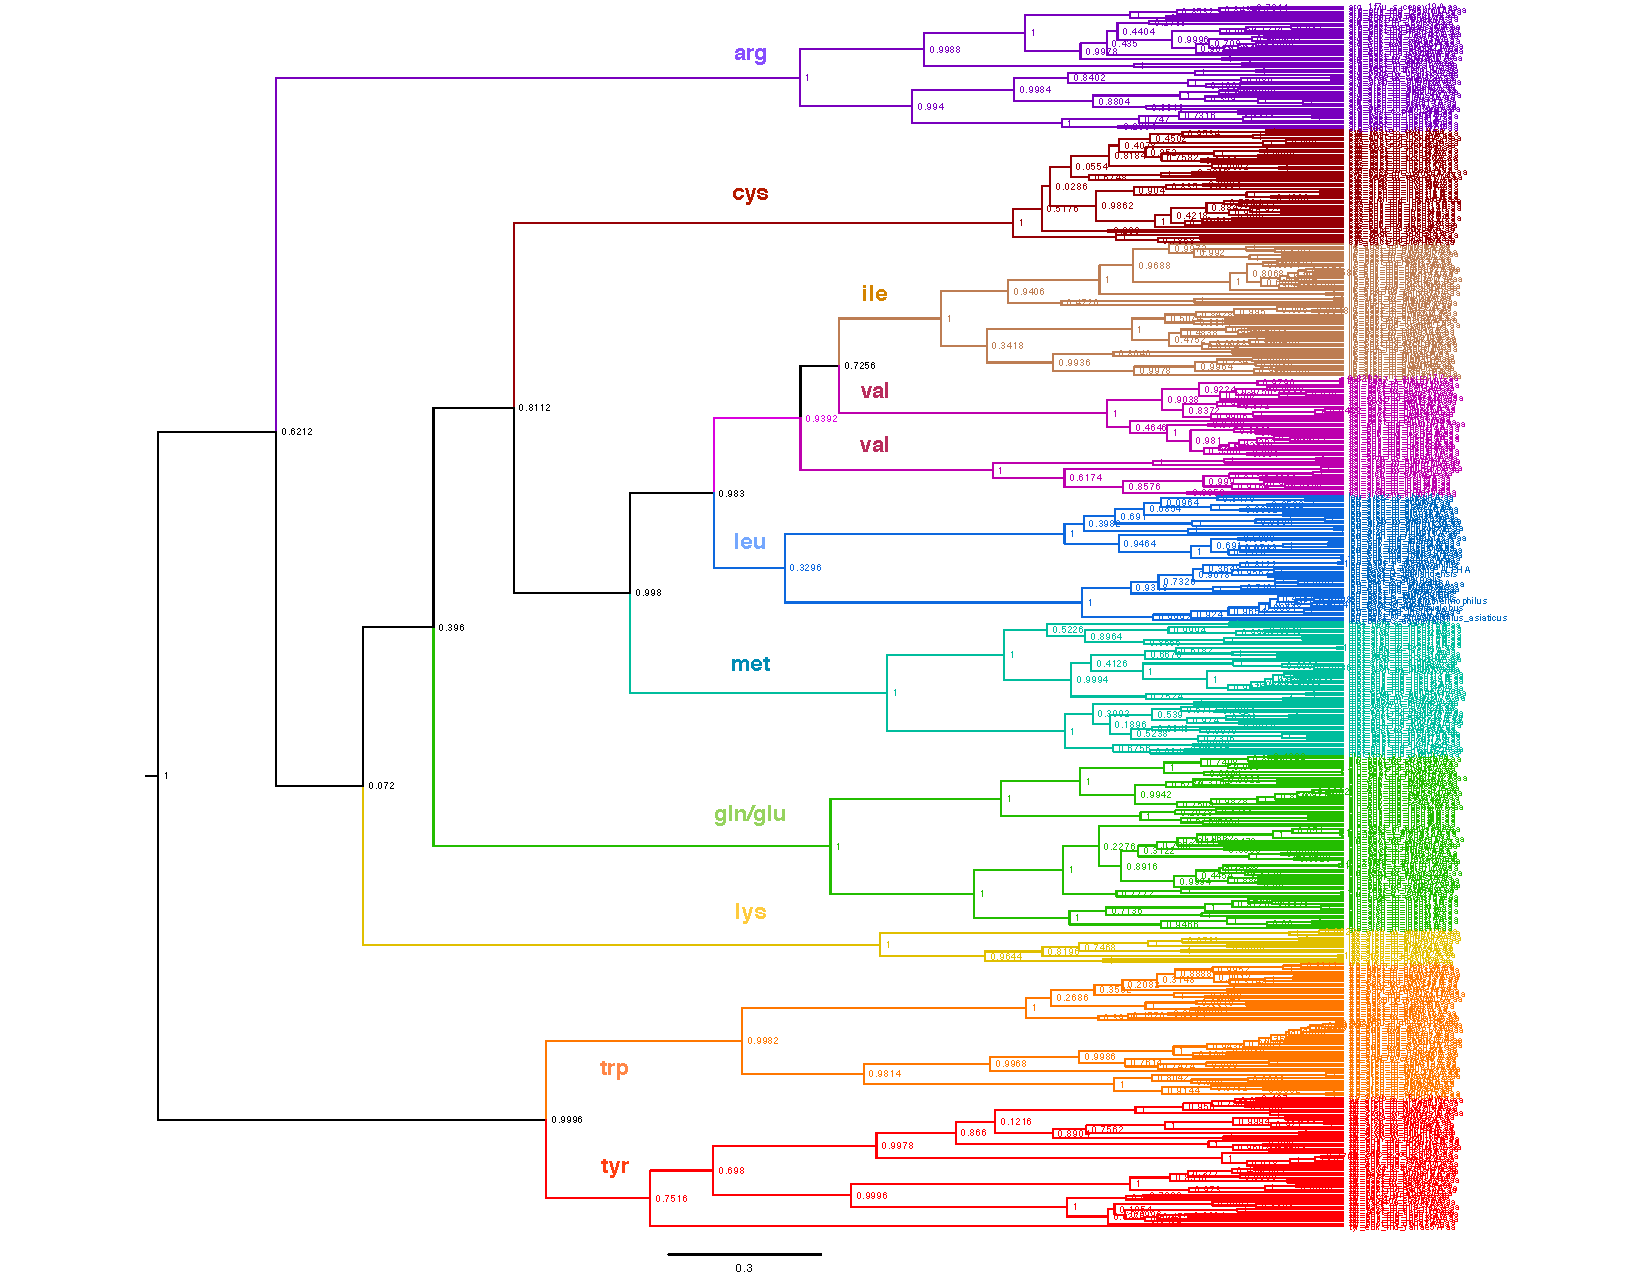
\includegraphics[width=\textwidth]{ClassI_Coalescent_1}
\end{figure}

% Either type in your references using
% \begin{thebibliography}{}
% \bibitem{}
% Text
% \end{thebibliography}
%
% or
%
% Compile your BiBTeX database using our plos2015.bst
% style file and paste the contents of your .bbl file
% here. See http://journals.plos.org/plosone/s/latex for 
% step-by-step instructions.
% 
\begin{thebibliography}{10}

% Use this sample article?? -could relate to Rodin-Ohno hypothesis

%\bibitem{bib1}
%G. C. Conant, K. H. Wolfe.
%\newblock {{T}urning a Hobby into a Job: How Duplicated Genes Find New
%  functions}.
%\newblock Nat Rev Genet. Dec;9(12):938--950. 2008.

% Modeller paper
\bibitem{bib1}
Webb B, Sali A.
\newblock Comparative protein structure modeling using Modeller.
\newblock Current Protocols in Bioinformatics, John Wiley and Sons, Inc., 5.6.1-5.6.32. 2014.

% 
\bibitem{bib2}
Marti-Renom MA, Stuart A, Fiser A, Sánchez R, Melo F, Sali A. 
\newblock Comparative protein structure modeling of genes and genomes.
\newblock Annu. Rev. Biophys. Biomol. Struct. 29, 291-325. 2000.

%
\bibitem{bib3}
Sali A, Blundell TL.
\newblock Comparative protein modelling by satisfaction of spatial restraints.
\newblock J. Mol. Biol. 234, 779-815. 1993.

% 
\bibitem{bib4}
Fiser A, Do RK, Sali A.
\newblock Modeling of loops in protein structures.
\newblock Protein Science 9. 1753-1773. 2000.

% HHpred paper
\bibitem{bib5}
Söding J, Biegert A, Lupas AN.
\newblock The HHpred interactive server for protein homology detection and structure prediction. 
\newblock Nucleic Acids Research. 33(Web Server issue):W244-W248. doi:10.1093/nar/gki408. 2005.

% POSA paper
\bibitem{bib6}
Li Z, Natarajan P, Ye Y, Hrabe T, Godzik A.
\newblock POSA: A user-driven, interactive multiple protein structure alignment server.
\newblock Nucl. Acids Res. 2014. doi: 10.1093/nar/gku394

% BEAST 2 paper
\bibitem{bib7}
Bouckaert R, Heled J, Kühnert D, Vaughan T, Wu C-H, Xie D, Suchard MA, Rambaut A, Drummond AJ.
\newblock BEAST 2: A software platform for Bayesian evolutionary analysis.
\newblock PLoS Computational Biology, 10(4), e1003537. 2014. doi:10.1371/journal.pcbi.1003537

% MCMC paper
\bibitem{bib8}
Drummond AJ, Nicholls GK, Rodrigo AG, Solomon S. 
\newblock Estimating mutation parameters, population history and genealogy simultaneously from temporally spaced sequence data.
\newblock Genetics 161, 1307-1320. 2002.

% Malaria (prolyl-) paper
\bibitem{bib9} 
Herman JD, Pepper LR, Cortese JF, Estiu G, Galinsky K, Zuzarte-Luis V, Derbyshire ER, Ribacke U, Lukens AK, Santos SA, Patel V, Clish CB, Sullivan Jr. WJ, Zhou H,
Bopp SE, Schimmel P, Lindquist S, Clardy J, Mota MM, Keller TL, Whitman M, Wiest O, Wirth DF, Mazitschek R. 
\newblock The cytoplasmic prolyl-tRNA synthetase of the malaria parasite is a dual-stage target of febrifugine and its analogs.
\newblock Science Translation Medicine, Vol 7, Issue 288. 2015.

% Woese paper
\bibitem{bib10} 
Woese CR, Olsen GJ, Ibba M, Soll D.
\newblock Aminoacyl-tRNA synthetases, the genetic code, and the evolutionary process.
\newblock Microbiology and Molecular Biology Reviews, p. 202-236. 2000.

% Wills paper - Emergence of Coding (intro to Remco's method)
\bibitem{bib11} 
Wills PR, Nieselt K, McCaskill JS.
\newblock Emergence of coding and its specificity as a physico-informatic problem.
\newblock Origins of Life and Evolution of Biospheres. 2015. doi:10.1007/s11084-015-9434-5.

% Rodin-Ohno paper
\bibitem{bib11} 
Rodin SN, Ohno S.
\newblock Four primordial modes of tRNA-Synthetase recognition, determined by the (G,C) operational code.
\newblock Proceedings of the National Academy of Sciences, Vol 94, pp. 5183-5188. 1997.

% Rodin-Ohno-Rodin paper
\bibitem{bib12} 
Rodin S, Ohno S, Rodin A.
\newblock Transfer RNAs with complementary anticodons: Could they reflect early evolution of discriminative genetic code adaptors?
\newblock Proceedings of the National Academy of Sciences, Vol 90, pp. 4723-4727. 1993.

% BOOK - CHECK CITATION FORMAT
\bibitem{bib13} 
Ibba M, Francklyn C, Cusack S.
\newblock The aminoacyl-tRNA synthetases.
\newblock Molecular Biology Intelligence Unit, Landes Bioscience. Georgetown, Texas, U.S.A. 2005.

% Molecular clock paper (longer time leads to genetic saturation)
\bibitem{bib14} 
Ho SY, Phillips MJ, Cooper A, Drummond AJ.
\newblock Time dependency of molecular rate estimates and systematic overestimation of recent divergence times.
\newblock Molecular Biological Evolution, 7:1561-8. 2005. doi: 10.1093/molbev/msi145.

% Molecular clock paper (relaxed clock)
\bibitem{bib15} 
Drummond AJ, Ho SYW, Phillips MJ, Rambaut A.
\newblock Relaxed phylogenetics and dating with confidence.
\newblock PLoS Biology, 4(5):e88. 2012. doi: 10.1073/pnas.1207965110.

% BDSKY paper
\bibitem{bib16} 
Stadler T, Kuhnert D, Bonhoeffer S, Drummond AJ.
\newblock Birth-death skyline plot reveals temporal changes of epidemic spread in HIV and hepatitis C virus (HCV).
\newblock Proceedings of the National Academy of Sciences of the United States of America, 110(1):228-33. 2013. doi: 10.1073/pnas.1207965110.

\end{thebibliography}


\end{document}

